\documentclass[11pt]{article}
% Nature Computational Science — Article (initial submission)
\usepackage[a4paper,margin=2.5cm]{geometry}
\usepackage[T1]{fontenc}
\usepackage[utf8]{inputenc}
\usepackage{lmodern}
\usepackage{amsmath,amssymb}
\usepackage{graphicx}
\usepackage{booktabs}
\usepackage{array}
\usepackage{caption}
\usepackage[super,sort&compress,comma]{natbib}
\usepackage{setspace}
\usepackage[mathlines]{lineno}
\usepackage{microtype}
\usepackage[hidelinks]{hyperref}
\usepackage{xcolor}

\DeclareCaptionLabelSeparator{bar}{\ $|$\ }
\captionsetup{font=small,labelfont=bf,labelsep=bar,justification=justified,singlelinecheck=false}
\renewcommand{\figurename}{Fig.}
\renewcommand{\tablename}{Extended Data Table}
\graphicspath{{../figures/}}
\setlength{\parskip}{0.35em}
\newcommand{\Dh}{\hat D}
\newcommand{\ReP}{\mathrm{Re}\,\Phi_0}
\newcommand{\ImP}{\mathrm{Im}\,\Phi_0}
\newcommand{\sstart}{s_{\mathrm{start}}}
\newcommand{\smax}{s_{\max}}

\begin{document}
\linenumbers
\onehalfspacing

\begin{center}
{\LARGE\bfseries A resonance phase locates unstable self-similar singularities beyond an exponential precision wall\par}
\vspace{1.2em}
{\large Ansh Mishra$^{1,*}$ and Aryan Senthilkumar$^{2}$\par}
\vspace{0.6em}
{\small $^{1}$Independent researcher.\quad $^{2}$Georgia Institute of Technology, Atlanta, GA, USA.\par}
\vspace{0.3em}
{\small $^{*}$Corresponding author.\par}
\end{center}

\vspace{1em}
\begin{abstract}
\noindent Unstable self-similar blow-up profiles of incompressible flow come in hierarchies, but their computable
depth is unknown. Here we show that direct computation meets an exponential precision wall: each profile is a zero of
a smoothness defect that shrinks about tenfold per profile. In incompressible porous-media flow, auditing every error
source reveals an erratic defect floor of $10^{-9}$. Two independent solvers agree to that floor, yet their profile
positions drift apart by five orders of magnitude, and a pre-registered holdout test could not identify the seventh
profile. A resonance phase, a quadrature over $O(1)$-accurate profile data, moves 10 to over 1,000 times less under
the same numerical changes, locates that profile ten times more precisely and predicts the wall through its
imaginary part. A tracking failure that passed residual checks was caught by a geometric invariant and repaired with
an exact scaling. Three deeper profiles are registered as benchmarks.
\end{abstract}

\section*{Main}

Whether the incompressible Euler equations can develop a singularity in finite time from smooth initial data is one
of the central open problems of mathematical physics. Near a solid boundary it has been resolved with computer
assistance: Luo and Hou observed explosive growth at the wall of a rotating cylinder\cite{luo2014}, and Chen and Hou
proved stable, nearly self-similar blow-up for the axisymmetric Euler equations and for their two-dimensional proxy,
the Boussinesq system with a boundary\cite{chen2022,chen2023}. Stable blow-up is, however, only the bottom of a
hierarchy. Physics-informed neural networks\cite{raissi2019,wang2023} have recently found the first few
\emph{unstable} self-similar profiles of the Boussinesq equations, of incompressible porous-media flow (IPM) and of
the C\'ordoba--C\'ordoba--Fontelos model\cite{wang2025,ccf2005}, and these profiles are now being computed towards
machine precision\cite{wang2025b}. Unstable profiles are the thresholds between qualitatively different evolutions
and the candidates for blow-up wherever the stable scenario is unavailable; computer-assisted proofs need them to
high accuracy\cite{chen2023,gomezserrano2019,buckmaster2022}. How deep such a hierarchy can be computed, and with
what certainty a computed profile is the profile it is claimed to be, are therefore computational questions with
mathematical consequences.

Here we show that these hierarchies carry an intrinsic obstruction, an exponential precision wall, and we give an
observable that removes it. The profiles are isolated members of a continuous branch of singular self-similar
solutions; each sits where a smoothness defect vanishes, and that defect is exponentially small in the profile
number. In IPM it falls about tenfold per profile, so each new profile demands ten times more precision. We audit
the complete error budget of a converged solver and find that, deep in the hierarchy, it is dominated by
discretization errors that are neither small nor smooth: a periodic locking of a receding front to the grid, an
angular-resolution error that stops converging, and round-off from deep origin truncation. An independent solver
confirms that the floor is a property of the problem, and a holdout test, pre-registered with a fixed decision
rule, shows its consequence: the seventh IPM profile cannot be identified by its defect.

The remedy is a different observable. The hierarchy is created by a short wave trapped in a stalled boundary layer,
and the smooth profiles are resonances of that wave. Its phase is a quadrature over $O(1)$-accurate profile data; it
is insensitive to the errors that dominate the defect, locates the seventh profile ten times more precisely, and its
imaginary part predicts the wall itself. We also report a failure of the phase computation that passed every
residual check, the geometric invariant that exposed it and the exact scaling that repaired it. Deeper in the branch
a steepening front limits the present method, and we leave the endpoint of the IPM hierarchy open while registering
three deeper profiles, with the precision a test would need, as a benchmark.

\subsection*{Smooth profiles are zeros of an exponentially small defect}

We seek self-similar solutions $\rho(x,t)=(1-t)^{\lambda}R(y)$, $y=x/(1-t)^{1+\lambda}$, of IPM on the half-plane
(Methods). For each blow-up rate parameter $\lambda$ there is a least-singular profile whose density behaves near the
stagnation point on the wall as $R\simeq c|y_1|^m$, with
\begin{equation}
m(\lambda)=\frac{\varepsilon}{1+\lambda-A(\lambda)},\qquad \varepsilon=\lambda ,
\label{eq:m}
\end{equation}
where $A$ is the strain at the stagnation point. The profile is smooth exactly when $m=2$. We follow this branch
continuously in $z=1/\lambda$ by Newton--Krylov continuation of a marching solver in log-polar coordinates
(Methods)\cite{keller1977,knoll2004} and locate the zeros of the defect $m-2$. Along the branch the self-similar
flow on the wall develops a slow layer, a dip and a receding front (Fig.~1a), which we return to below.

Along the branch the defect oscillates with an amplitude that falls geometrically (Fig.~2a). Its extrema are
$8.05\times10^{-2}$, $7.70\times10^{-3}$, $7.71\times10^{-4}$, $7.55\times10^{-5}$, $7.04\times10^{-6}$,
$5.45\times10^{-7}$ and $5.07\times10^{-8}$, falling by a factor of 10.0--12.9 per half-period. At its zeros, the
smooth profiles $\lambda_1,\dots,\lambda_7$, the defect crosses zero with slopes $|dm/dz|=5.4\times10^{-2}$,
$5.9\times10^{-3}$, $6.4\times10^{-4}$, $6.6\times10^{-5}$, $6.6\times10^{-6}$, $4.6\times10^{-7}$ and
$2.5\times10^{-8}$. A zero located from a defect known to $\pm\sigma_m$ is uncertain by $\sigma_z=\sigma_m/|dm/dz|$,
so any fixed error floor is overtaken and $\sigma_z$ grows by a factor of 10--20 per profile (Fig.~2c). The precision
needed to locate profile $n$ is set by the profile number, not by the order of the method. Defects that are beyond
all orders in a small parameter\cite{boyd1999,kruskal1991,berry1989} are the rule for hierarchies generated by a slow
layer; the 2D Boussinesq and Hou--Luo hierarchies behave in the same way (Supplementary Note~1).

\begin{figure}[t]
\centering
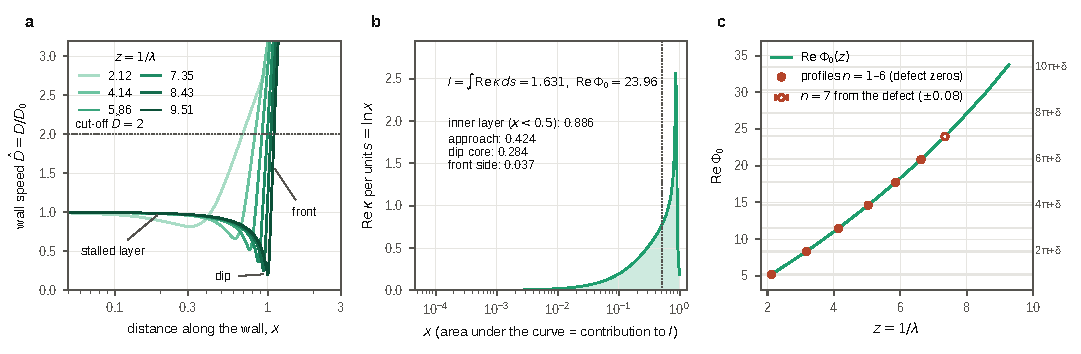
\includegraphics[width=\textwidth]{Fig1.pdf}
\caption{\textbf{The object and the observable (IPM).} \textbf{a}, Wall speed $\Dh=D/D_0$ along the wall for
profiles of increasing depth $z=1/\lambda$: a stalled layer ($\Dh\approx1$), a dip that deepens, and a front that
recedes. Dotted line: the front cut-off of the phase. \textbf{b}, Integrand $\mathrm{Re}\,\kappa$ of the resonance
phase per unit $s=\ln x$ at $z=7.346$ (logarithmic $x$ axis, so area is contribution), with the partition of
$I=D_0\ReP$ into inner layer, approach, dip core and front side. \textbf{c}, $\ReP$ along the branch against the
levels $n\pi+\delta$ ($\delta=2.031$). Filled symbols: profiles $n=1$--6 located as zeros of the defect; open
symbol: $n=7$ with the systematic uncertainty of the defect.}
\label{fig:1}
\end{figure}

An independent solver sees the same wall. A global sparse Newton solver that shares no numerical ingredient with the
marching solver imposes $m=2$ directly and treats $\lambda$ as an eigenvalue (Methods). It reproduces the IPM profiles
$n=1$--6 to $|\Delta\lambda|=1.4\times10^{-8}$, $3.7\times10^{-8}$, $3.4\times10^{-8}$, $6.5\times10^{-7}$,
$9\times10^{-7}$ and $1.3\times10^{-4}$. Converted with the measured crossing slopes, every one of these differences
corresponds to $0.2$--$3.5\times10^{-9}$ in $m$: the two solvers agree to the same floor in the defect at every
depth, while their disagreement in profile position grows by five orders of magnitude (Fig.~2c). The wall is a
property of the problem, not of a solver. The same pair of solvers reproduces all eight smooth profiles of the 2D
Boussinesq system to $10^{-5}$ (Supplementary Note~1).

\begin{figure}[t]
\centering
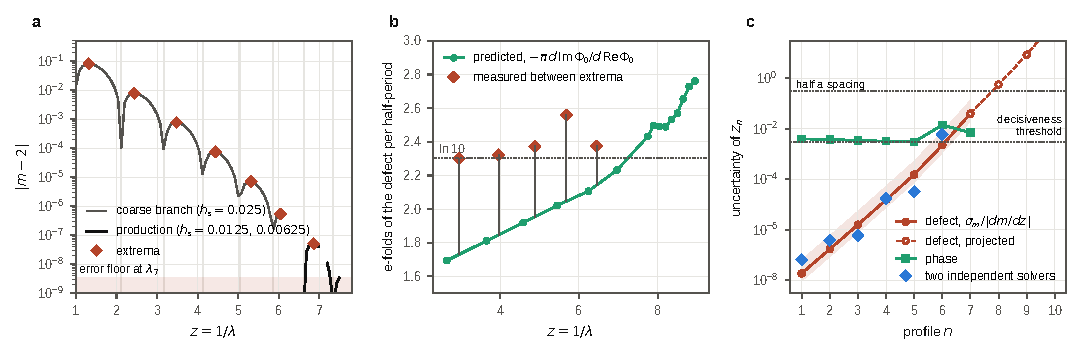
\includegraphics[width=\textwidth]{Fig2.pdf}
\caption{\textbf{The exponential precision wall.} \textbf{a}, $|m-2|$ along the IPM branch (coarse branch,
$h_s=0.025$; production scans, $h_s=0.0125$ and $0.00625$) and its extrema, which fall tenfold per half-period,
against the error floor at $\lambda_7$. Vertical lines: the profiles. \textbf{b}, Decay of the defect per
half-period predicted by the imaginary part of the phase, $-\pi\,d\ImP/d\ReP$, against the decay between consecutive
extrema; the difference is $(0.7$--$1.4)\lambda$ times the prediction. \textbf{c}, Uncertainty of the profile
position $z_n$: from the defect at a fixed floor $\sigma_m=10^{-9}$ (band, $0.5$--$3.4\times10^{-9}$; measured
crossing slopes for $n\le7$, projected beyond), from the phase (offset scatter and grid error divided by
$d\ReP/dz$), and the difference between two independent solvers.}
\label{fig:2}
\end{figure}

\subsection*{An audit of the error floor}

We audited every numerical parameter at the deepest profiles (Fig.~3 and Extended Data Table~1). The production settings are
angular collocation with $N_b=32$ points, radial spacing $h_s=0.0125$ in $s=\ln r$, origin truncation $\sstart=-20$,
far field at $\smax=100$ and a Newton tolerance near the residual floor. Three findings matter beyond this problem.

\emph{Front--grid locking.} As $\lambda$ decreases, a front on the wall recedes across the radial grid and modulates
$m$ with the period of one grid cell in the front's position. We measured the modulation directly by solving the
same $\lambda$ on grids shifted by $\tfrac14$, $\tfrac12$ and $\tfrac34$ of a cell (Supplementary Note~2 and
Supplementary Fig.~1). Its half-range is
$1.5\times10^{-6}$, $1.2\times10^{-8}$ and $8\times10^{-11}$ at $h_s=0.025$, $0.0125$ and $0.00625$, falling as
$h_s^{7.1}$ (Fig.~3a). Averaging over the four shifts cancels its first three harmonics. On the coarsest grid it
produced a spurious zero of $m-2$ at $z=6.905$ and displaced the sixth profile by $0.037$ in $z$, or 5\% of a
spacing. A plausible-looking but spurious profile is the characteristic failure of direct location.

\emph{Angular resolution stops converging.} At the seventh profile ($z=7.346$, $h_s=0.00625$), $m-2$ moves by
$-1.1\times10^{-9}$ from $N_b=32$ to $48$ and by a further $-2.3\times10^{-9}$ from $48$ to $64$, whereas at the
sixth profile $N_b=48\to64$ changes $m$ by only $9\times10^{-11}$. The floor is erratic, not a convergent tail that
extrapolation could remove.

\emph{Deeper truncation is not better.} Starting the march from the exact local solution at $\sstart$ leaves an
offset that decays roughly as $e^{\sstart}$, from $2.1\times10^{-8}$ at $-15$ to $2.2\times10^{-10}$ at $-19$
(Fig.~3c). Beyond about $-20$ two errors grow instead: the converged Newton residual, from
$0.4$--$2\times10^{-13}$ at $-16$ to $-18$ through $5\times10^{-13}$ at $-20$ to $1.9\times10^{-12}$ at $-26$ and
$1.5\times10^{-11}$ at $-30$ (Fig.~3d), and a round-off offset in $m$ of $1.5\times10^{-9}$ at $-24$ (identical at the
fifth and seventh profiles, hence independent of $\lambda$), $7.7\times10^{-9}$ at $-26$ and $2.1\times10^{-8}$ at
$-30$, as large as the truncation error at $-15$.

Together these give an erratic floor of $1$--$3\times10^{-9}$ in $m$ at the seventh profile. The Newton floor
($\lesssim10^{-12}$) and the far field ($\smax=100\to160$: $6\times10^{-12}$, after a path-dependent
$6\times10^{-10}$ at $130$) are smaller.

\begin{figure}[t]
\centering
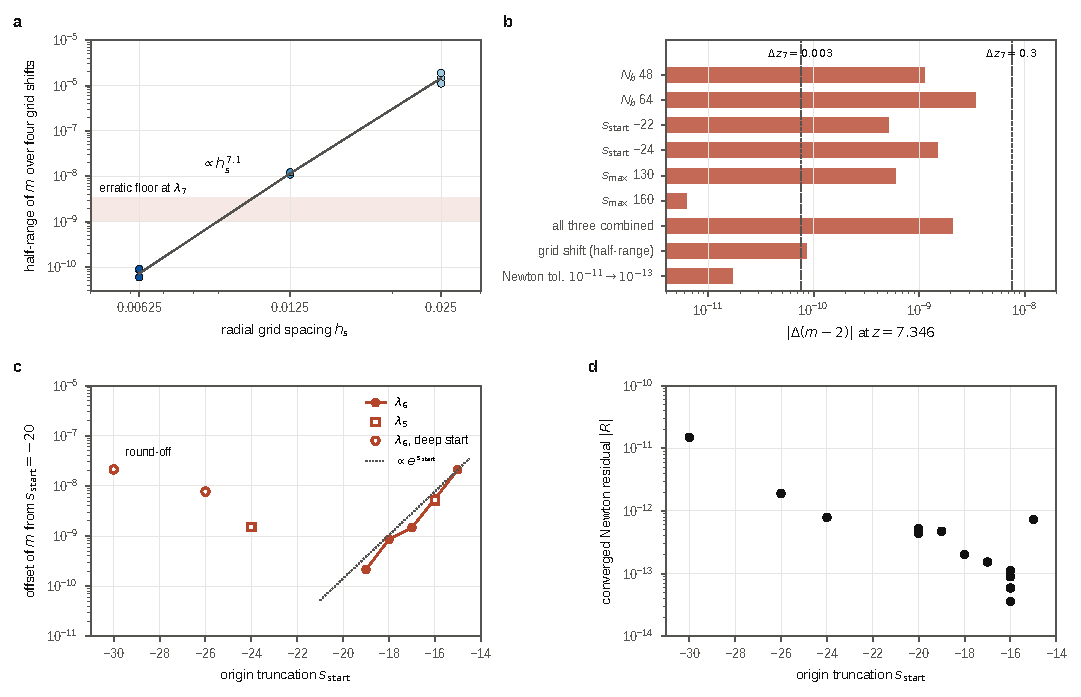
\includegraphics[width=\textwidth]{Fig3.pdf}
\caption{\textbf{Anatomy of the error floor.} \textbf{a}, Half-range of $m$ over four grid shifts against the radial
spacing $h_s$ at $z=7.26$--$7.38$: front--grid locking falls as $h_s^{7.1}$. \textbf{b}, Change of $m$ at the seventh
profile under each audited parameter (production state $h_s=0.00625$), against the changes that would move $z_7$ by
$0.003$ and $0.3$. \textbf{c}, Offset of $m$ against the origin truncation $\sstart$: it decays as $e^{\sstart}$ down
to $-19$; deeper starts add a round-off offset. \textbf{d}, Converged Newton residual against $\sstart$.}
\label{fig:3}
\end{figure}

\subsection*{A pre-registered holdout the defect cannot decide}

We used the deepest profile that the error budget allows as a holdout. Before any fine-grid computation below the
sixth profile, we committed five predictions for $z_7=1/\lambda_7$ to a public repository: four from rules fitted to the
lower profiles (a shifted law fitted to two ranges, a geometric contraction and a three-point law; git commit
\texttt{c922751}) and one from the resonance phase evaluated on a coarse branch (\texttt{273ae28}). The decision rule, also fixed before
the crossing was known (\texttt{f0b3f06}), disfavours a hypothesis that misses by more than $2\sigma$, counts the
comparison as decisive only if $\sigma_z\le0.003$ (small enough to separate the two families of predictions, $0.007$
apart, at $2\sigma$), and takes the measured value from matched scans at two resolutions (Extended Data Table~2, Fig.~4 and
Supplementary Note~3).

The committed procedure could not run as written, because its $h_s=0.0125$ scan had been paused to test the locking
error; this deviation is recorded. On the converged grid ($h_s=0.00625$, four shifts per point) the defect gives
$z_7=7.3451\pm0.0016$ (statistical). The systematic variants at the crossing move $z_7$ by $-0.045$ ($N_b=48$),
$-0.137$ ($N_b=64$), $-0.021$ and $-0.060$ ($\sstart=-22$, $-24$), $+0.024$ ($\smax=130$) and $-0.083$ (all three
together), so that $z_7=7.35\pm0.08$. Every registered prediction lies within $0.2\sigma$ and $\sigma_z$ exceeds the
decisiveness threshold about 25-fold; as the rule requires, the holdout is recorded as not decisive and no
hypothesis is preferred. Five predictions spanning $0.018$ in $z$ cannot be told apart even though every solve reaches
a Newton residual below $10^{-12}$: the defect has run out of significant digits one profile after the sixth, where
$\sigma_z$ was $0.002$.

\begin{figure}[t]
\centering
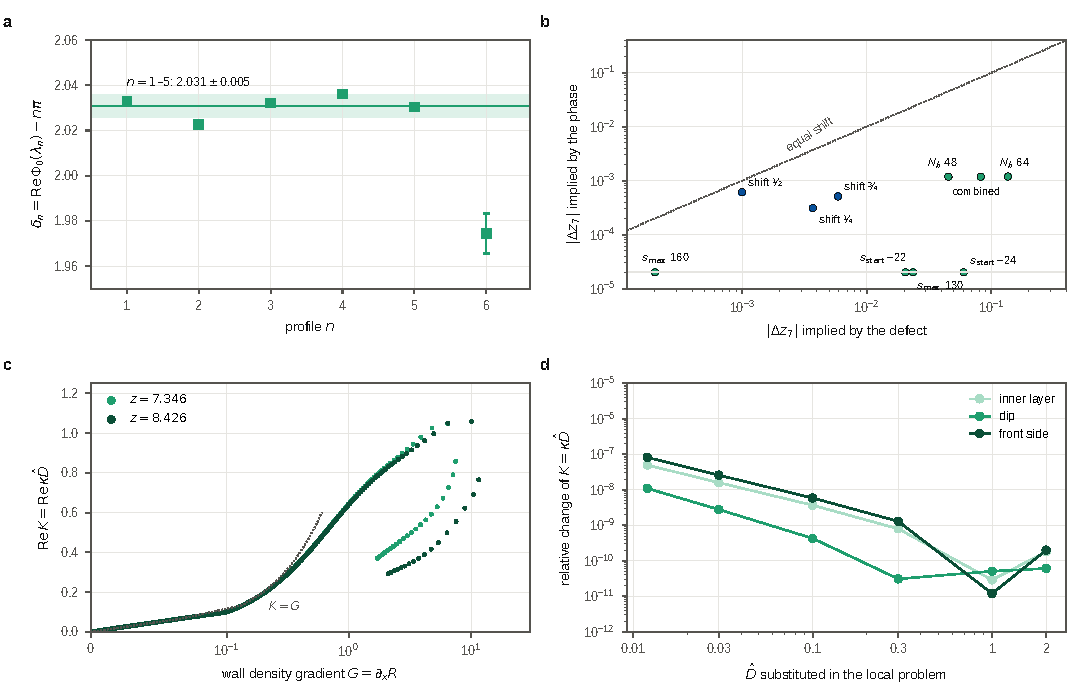
\includegraphics[width=\textwidth]{Fig4.pdf}
\caption{\textbf{The seventh profile: a pre-registered holdout.} Predictions registered before the computation
(triangles; git commits in parentheses), the measurement from the defect (thick bar: statistical, $\pm0.0016$; thin
bar: systematic, $\pm0.08$), the decisiveness threshold of the registered rule (grey band, $\pm0.003$) and the
unregistered reading of the resonance phase (green, $z_7=7.354\pm0.007$).}
\label{fig:holdout}
\end{figure}

\subsection*{A resonance phase that bypasses the wall}

The hierarchy has a physical origin. As $\varepsilon$ decreases, the self-similar flow along the wall stalls in a
layer between the stagnation point and a front (Fig.~1a). Perturbations travel through this layer as short waves,
$\exp(i\int\kappa\,ds/D_0)$, with $s=\ln x$ and $D_0=\varepsilon/m$ the stagnation-point value of the wall speed
$D=V_1/x$. The local wavenumber $\kappa(s)$ is the root of an ordinary-differential eigenproblem across the layer at
each wall point (Methods), and the smooth profiles are resonances of the wave:
\begin{equation}
\ReP(\lambda_n)=n\pi+\delta ,\qquad \Phi_0=\frac{1}{D_0}\int\kappa\,ds ,
\label{eq:res}
\end{equation}
integrated from the stagnation point to the front cut-off $D/D_0=2$ (Fig.~1c and Supplementary Note~4). Three
properties make $\Phi_0$ a computational observable.

\emph{It is a quadrature over $O(1)$ data.} The local problem needs only the wall data of the profile --- the wall
speed, its strain $\mu$ and the density gradients $G=\partial_xR$ and $R_y$ --- none of which is exponentially small;
$\Phi_0$ inherits the relative accuracy of the profile, not that of the defect. At the seventh profile the inner layer
($x<0.5$) contributes $0.886$ of $I=D_0\ReP=1.631$, and the receding outer structure the rest (Fig.~1b).

\emph{It has an exact scaling.} In IPM the vorticity is slaved to the density gradient, $\Omega=-\partial_1R$.
Rescaling the wall-normal coordinate by $\Dh=D/D_0$ removes the wall speed from the local problem, so that
\begin{equation}
\kappa=\frac{K(G,\mu,R_y)}{\Dh},\qquad \Phi_0=\int\frac{K}{D}\,ds .
\label{eq:scaling}
\end{equation}
Numerically $K$ is invariant to $10^{-7}$ when $\Dh$ is varied from $0.012$ to $2$ at fixed $(G,\mu,R_y)$
(Fig.~5d). $K\approx G$ for small $G$ and levels off at $0.8$--$1.05$ for $G\gtrsim3$ on the approach and the dip
(Fig.~5c), so $\Phi_0$ is close to a weighted travel time $\int ds/D$, a geometric property of the stalled layer:
along the branch $I=0.76\,T+\text{const}$ for the shallow profiles and $0.81\,T+\text{const}$ for the deep ones, with
$T=\int ds/\Dh$.

\emph{It is stable where the defect is not.} We recomputed $\Phi_0$ on every variant state of the audit at the
seventh profile (Fig.~5b and Extended Data Table~1). Changes that move $z_7$ by up to $0.137$ through the defect move it by at most
$0.0012$ through the phase. $N_b=32\to48$ shifts $\ReP$ once by $0.005$, after which $N_b=48$ and $64$ agree to
$10^{-4}$ while the defect keeps moving; $\sstart$ and $\smax$ change $\ReP$ by less than $5\times10^{-5}$
($\Delta z<10^{-5}$) against $0.02$--$0.06$ through the defect; grid shifts change it by at most $0.003$
($\Delta z\le0.0006$) against up to $0.006$. The phase moves 10 to more than 1,000 times less than the defect.

\begin{figure}[t]
\centering
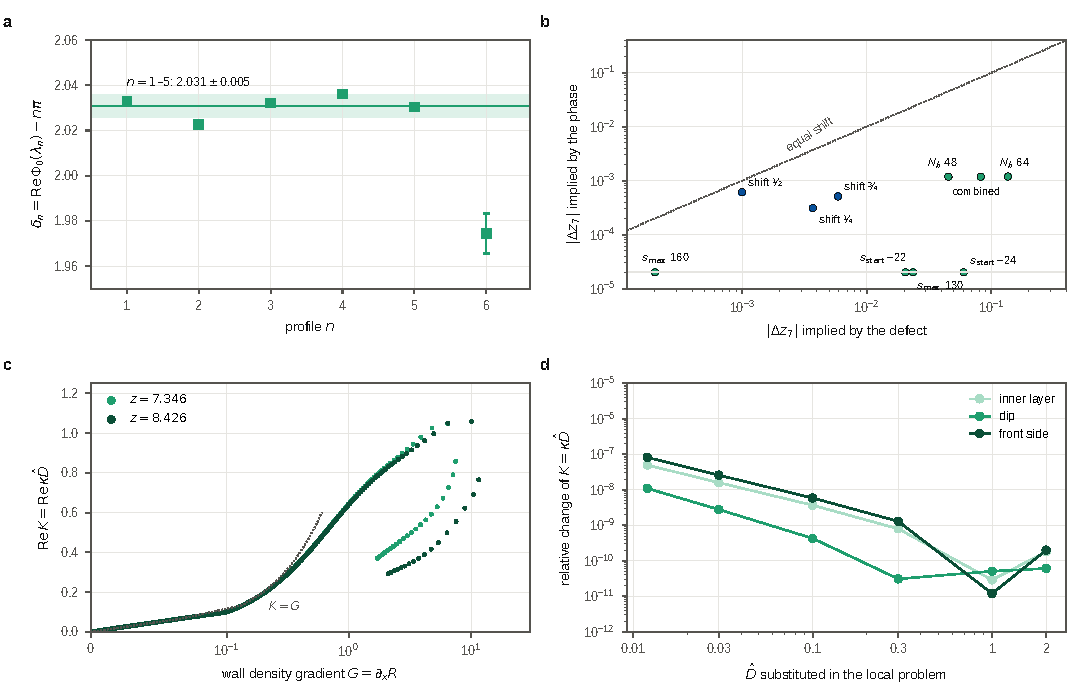
\includegraphics[width=\textwidth]{Fig5.pdf}
\caption{\textbf{The phase is stable where the defect is not.} \textbf{a}, Offsets $\delta_n=\ReP(\lambda_n)-n\pi$:
$2.031\pm0.005$ for $n=1$--5 (band) and $1.974\pm0.009$ at $n=6$. \textbf{b}, For every audited change at the
seventh profile, the shift of $z_7$ implied by the phase against that implied by the defect; changes below
$2\times10^{-5}$ are drawn at that value. Dotted: equal shift. \textbf{c}, $\mathrm{Re}\,K=\mathrm{Re}\,\kappa\Dh$
against the wall density gradient $G$ along two profiles. \textbf{d}, Exact scaling: relative change of $K$ when the
local problem is solved with $\Dh$ replaced by $0.012$--$2$ at fixed $(G,\mu,R_y)$, at three wall points.}
\label{fig:phase}
\end{figure}

The offsets $\delta_n=\ReP(\lambda_n)-n\pi$ are $2.0331$, $2.0227$, $2.0320$, $2.0360$ and $2.0301$ for $n=1$--5,
constant to $\pm0.005$ (0.2\% of a spacing) with no adjustable parameter beyond the cut-off (Fig.~5a). At $n=6$ the
offset is $1.974\pm0.009$, a drift of $-0.057$ that we carry as an uncertainty. The drift is not an artefact of the
cut-off: with cut-offs $D/D_0=1.5$, $3$ and $5$ the offsets trend differently over $n=1$--5, but each drops by an
extra $0.04\pm0.01$ at $n=6$ (Supplementary Note~4). At the seventh profile the phase reads $z_7=7.354\pm0.007$, the
range spanned by $\delta=1.974$ and $2.031$; this is more than ten times tighter than the defect and consistent with it. The
grid dependence of $\ReP$ at that depth is $0.010$ ($\Delta z=0.002$). This reading is not one of the registered
predictions; the registered phase rule, evaluated on a coarser branch with an earlier tracker, gave $7.352$.

The imaginary part of the same quadrature predicts the wall (Fig.~2b). If the defect behaves as
$|A|e^{-|\ImP|}\cos(\ReP+\arg A)$\cite{bender1978,chapman1998}, its envelope decays by $e^{-|\Delta\ImP|}$ per
half-period. From the computed phase, $-\pi\,d\ImP/d\ReP=1.73$, $1.85$, $1.95$, $2.05$ and $2.15$ e-folds per
half-period at $z=3.0$--$6.5$, against measured decays of $2.30$, $2.32$, $2.37$, $2.56$ and $2.38$. The deficit is
$(0.7$--$1.4)\lambda$ times the prediction, the size of the $O(\lambda)$ corrections omitted at leading order. The
precision that a direct method needs at profile $n$ is therefore itself computable from the same $O(1)$ quadrature
that locates the profile. The phase has a second, physical role that we use only as a consistency check: in 2D
Boussinesq and the Hou--Luo model\cite{choi2017} it also quantizes the unstable spectrum of the profiles, and the
$n$-th profile has exactly $n$ unstable directions (Supplementary Note~1).

\subsection*{A failure that passed every residual check}

The phase requires one root $\kappa(s)$ of the local eigenproblem to be tracked along the wall, and this tracking
failed in a way that residuals could not reveal. On the deep states ($z>7.5$) the wall speed rises from $\Dh\approx0.3$
at the dip to $2$ at the cut-off within a few tracking steps, and $\kappa$ changes by the same factor. The original
tracker predicted each root from the previous $\kappa$, missed it, and on failure held $\kappa$ fixed, which inflates
$K=\kappa\Dh$ in proportion to $\Dh$ (Fig.~6a): at $z=7.946$, $K$ reached $5.4-5.6i$ at the cut-off where the
continued root is $0.33-0.10i$, and $I$ was 14\% too high --- an error of $3.7$ in $\ReP$, more than one profile
spacing. Every value returned was a genuine root of the local problem or a held value, two roots lie close together on
the front side, and every profile had a Newton residual below $10^{-12}$. The tracker did count its failed points, zero
on every shallow state and two to four on every deep one, but it carried on, because on the shallow states such
points had been harmless.

The error was exposed by geometry. The old $I(z)$ was non-monotone ($1.659$, $1.723$, $1.746$, $1.921$, $1.747$,
$1.856$, \dots) whereas the travel time $T$ of the same profiles grows smoothly (Fig.~6b). The repair uses the exact
scaling~(\ref{eq:scaling}): beyond the dip the tracker continues $K$ rather than $\kappa$, with predictor
$K_{\mathrm{prev}}/\Dh$ on a four times finer step, accepts a root only if $K$ is continuous to 25\%, holds $K$ (not
$\kappa$) at a failed point, and excludes any state with a failed point. It reproduces the shallow values
($\ReP=11.4568$ against $11.4566$ at $n=3$) and removes the jump; one of 17 deep states ($z=9.386$, 11 failed points)
is excluded (Supplementary Note~5). Three lessons generalize: residuals certify roots, not branches; exact invariances provide both
predictors and validators; and failure counters must gate results, not only log them. The failure and its repair are
part of the pre-registration record.

\begin{figure}[t]
\centering
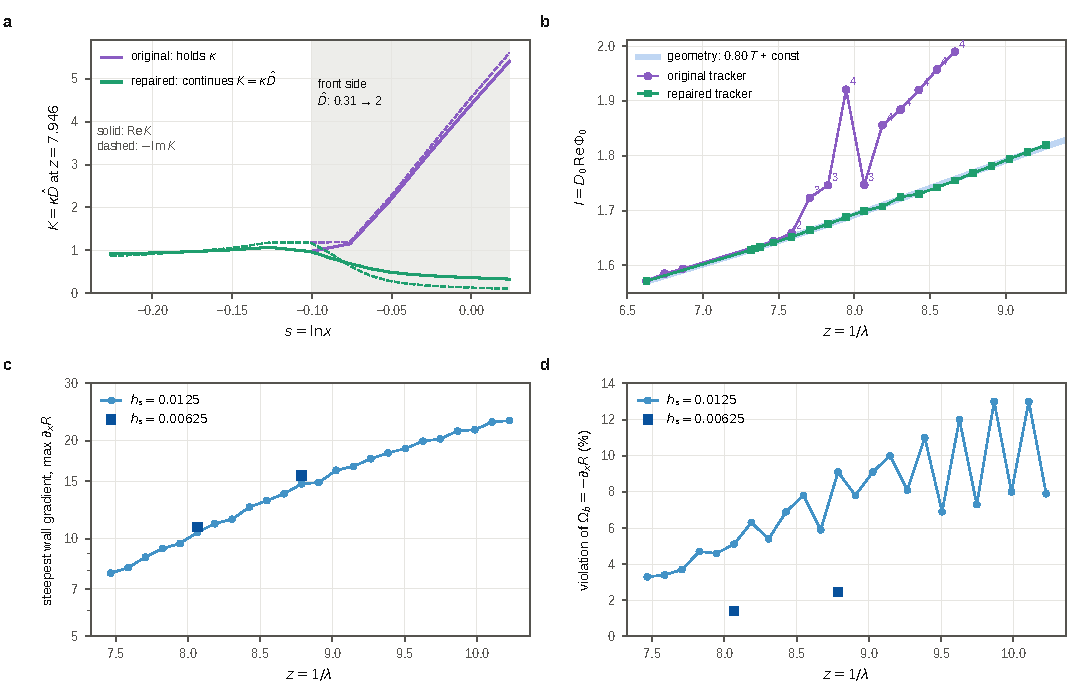
\includegraphics[width=\textwidth]{Fig6.pdf}
\caption{\textbf{A failure that residuals missed, and the deep branch.} \textbf{a}, $K=\kappa\Dh$ along the front
side of the deep state $z=7.946$ (shaded): the original tracker holds $\kappa$, so $K$ grows with $\Dh$; the repaired
tracker continues $K$. Solid, $\mathrm{Re}\,K$; dashed, $-\mathrm{Im}\,K$. \textbf{b}, $I=D_0\ReP$ from both trackers
against the geometric travel time ($0.80\,T+\text{const}$); numbers: points the original tracker counted as failed
but carried on. \textbf{c}, Steepest density gradient on the front side along the deep branch, at $h_s=0.0125$ and in
two checks at $h_s=0.00625$. \textbf{d}, Violation of the exact identity $\Omega_b=-\partial_xR$ (resolution
indicator).}
\label{fig:6}
\end{figure}

\subsection*{The deep branch and an open endpoint}

Following the branch to $z=10.23$ ($\lambda=0.098$) on $h_s=0.0125$ shows why the endpoint of the IPM hierarchy is
beyond the present method (Fig.~6c,d, Supplementary Note~6 and Supplementary Fig.~2). The dip in the wall speed deepens ever more slowly:
$\Dh_{\min}$ falls from $0.36$ to $0.20$ between $z=7.47$ and $9.51$, at $0.107$ per unit $z$ early and $0.045$ over
the last unit, and stays at $0.19\pm0.01$ out to $z=10.23$, while the dip and the front recede ($x_{\mathrm{dip}}$
from $0.88$ to $1.00$). The front steepens: the largest density gradient on the wall rises from $7.8$ to $23$, and the
violation of the exact identity $\Omega_b=-\partial_xR$, our resolution indicator, grows from 3\% to 7--13\% at
$h_s=0.0125$. Halving $h_s$ at $z=8.066$ and $8.786$ leaves $\Dh_{\min}$, the dip and front positions and $T$
unchanged to 0.3\%, lowers the indicator from 5.1\% and 9.1\% to 1.4\% and 2.5\%, raises the largest gradient by
4--6\% and $\ReP$ by $0.037$ and $0.017$ ($\Delta z\le0.007$), and reduces $m-2$ from $2.4\times10^{-8}$ and
$3.3\times10^{-7}$ to $1.0\times10^{-9}$ and $2.0\times10^{-9}$. Between these two depths, about one profile spacing
apart, the error of the defect at fixed $h_s$ grows fourteenfold while the signal falls about fifteenfold. The
geometry is resolved and the slowing of the dip is real; it is the steepening front that demands resolution, faster
than a uniform grid supplies it.

Along the branch the phase coefficient $I$ grows linearly, with slope $0.098$ per unit $z$ and a weak positive
curvature ($+0.005\pm0.002$) over $7.47\le z\le9.27$. A saturating $I$, the case of a stalled layer of fixed extent as
in the 2D Boussinesq and Hou--Luo hierarchies (Supplementary Fig.~3), is therefore excluded. Three continuations remain consistent with the
data: $I$ keeps growing linearly, so that profiles accumulate at $\lambda=0$ with $\lambda_n\propto n^{-1/2}$; $I$
diverges at a finite $z_c$, so that profiles accumulate at $\lambda_c=1/z_c>0$; or the branch terminates at a singular
front with a finite phase. Pole and logarithmic fits over the full range prefer $z_c\approx10$--$13$ but with
$\chi^2\approx35$ for 20 degrees of freedom, the deep range alone admits any $z_c\ge9.5$, and linear extrapolations of
$\Dh_{\min}$ and of the inverse largest gradient over the last unit vanish only near $z\approx18$ and $13$ and
continue to decelerate. We therefore record the endpoint class of the IPM hierarchy as unresolved; deciding it needs a
mesh that follows the front.

Within the computed range the phase still predicts profiles. Before any test we registered $\lambda_8$, $\lambda_9$ and
$\lambda_{10}$ from equation~(\ref{eq:res}) (git commit \texttt{251bf1e}), each with a band that covers the possible
drift of $\delta$, the measured grid correction and the smoothing error, and with the precision that a decisive test
($\sigma_z\le0.01$) needs according to the decay rate predicted by $\ImP$: $z_8=7.999$ $[7.970,8.017]$ needs
$\sigma_m\lesssim2\times10^{-11}$, $z_9=8.628$ $[8.590,8.645]$ needs $\sigma_m\lesssim1\times10^{-12}$ and
$z_{10}=9.201$ $[9.158,9.214]$ needs $\sigma_m\lesssim6\times10^{-14}$, below what a double-precision solver of this
kind delivers (Extended Data Table~2). The band at $n=8$ contains the rule-based predictions registered earlier and excludes the
earlier phase rule, which had been evaluated with the faulty tracker. The values of $m-2$ that we had computed in this
range lie at or below the floor; they are disclosed in the record and carry no information.

\section*{Discussion}

Hierarchies of unstable self-similar solutions generated by a slow layer have smoothness defects that are beyond all
orders in the layer parameter. Any method that locates them as zeros of the defect pays a precision cost that grows
exponentially with depth, and this holds for neural solvers as much as for classical ones. The residual that a solver
reports does not measure this cost: our profiles have residuals of $10^{-13}$, while their defects are decided at
$10^{-9}$.

The remedy is to change the observable rather than the solver. An asymptotic invariant of the mechanism --- here a
WKB phase --- converts an exponentially ill-conditioned root search into a well-conditioned quadrature; its imaginary
part prices the wall in advance, and its exact symmetries supply the predictors and validators that make it robust.
The construction applies wherever a hierarchy arises from a stalled or slow region, for example in other
boundary-driven blow-up scenarios\cite{chen2021cmp,kiselev2014} and in self-similar solutions of compressible and
dispersive equations\cite{merle2022,eggers2015}.

Three practices that we used are cheap and transferable\cite{peng2011,stodden2016}. Pre-registration with fixed
decision rules\cite{nosek2018} turned an inconclusive computation into a reportable negative result instead of a
post-hoc fit. Measuring periodic discretization errors by grid shifting exposes a locking error that convergence
studies at a fixed grid offset cannot see. Cross-checking a derived observable against an independent geometric proxy
caught a failure that residuals missed.

Our study has limitations. The resonance condition is derived by formal matched asymptotics and is not proved. The
offset $\delta$ drifts by $0.057$ at the sixth profile, which limits the phase to about 1\% of a spacing deep in the
ladder. The independent global solver confirms the IPM profiles only to its own floor in the defect, and its finer
grids did not converge at $\lambda_5$ and $\lambda_6$; the deepest IPM computations rest on one solver family with
extensive internal variants. The endpoint of the IPM hierarchy is open, and the registered profiles $\lambda_8$--$\lambda_{10}$
await a solver with a front-adapted mesh and, for $\lambda_{10}$, extended precision.

\section*{Methods}

\paragraph{Self-similar formulation.} In self-similar variables $y=x/(1-t)^{1+\lambda}$ and $\tau=-\ln(1-t)$, a
self-similar IPM density $\rho=(1-t)^{\lambda}R(y)$ satisfies $V\cdot\nabla R=\lambda R$ with $V=(1+\lambda)y+U$,
$U=\nabla^{\perp}\Psi$ and $-\Delta\Psi=\Omega=-\partial_1R$ on the half-plane with no penetration. By symmetry the
problem is posed on the quarter plane, in log-polar coordinates $(s,\beta)$ with $s=\ln r$ and $\beta=0$ the wall.
The least-singular profile is normalized at the stagnation point, where $R\simeq|y_1|^m$ with $m$ given by
equation~(\ref{eq:m}) and $A=-\partial_1U_1(0)$. The 2D Boussinesq and Hou--Luo formulations used for validation are
given in Supplementary Note~7.

\paragraph{Marching solver.} The stagnation-point structure is factored out, $R=\cos^m\!\beta\,\hat R$. Since all
characteristics leave the origin, $\hat R$ is marched outwards in $s$ from the exact local solution at $\sstart=-20$
(implicit two-stage Gauss--Legendre for $s<12$, classical Runge--Kutta beyond)\cite{hairer1993,hairer1996}. The
velocity is obtained from $X=\Psi/r^2$ by eighth-order finite differences in $s$\cite{fornberg1988} and Chebyshev
collocation in $\beta$\cite{trefethen2000} with $N_b=32$, on $s\in[-120,100]$. The fixed point $X=\mathcal{B}(\mathrm{march}(X))$
of the march and the Biot--Savart map $\mathcal{B}$ is solved by Newton--Krylov iteration (GMRES\cite{saad1986}) with
central-difference Jacobian--vector products, which converges quadratically to residuals of $4$--$8\times10^{-13}$.
The branch is followed in $z=1/\lambda$ with secant predictors, and profiles are located by secant iteration on
$m(\lambda)=2$ and by scans on fixed $z$ grids. One solve takes 3--8 min at $h_s=0.0125$ and 11--23 min at
$h_s=0.00625$ on one core.

\paragraph{Independent global solver.} The unknowns are the unfactored fields $(R,\Omega,X)$ on the $(s,\beta)$ grid,
solved simultaneously with sixth-order finite differences in $s$ (upwind-biased for transport) and Chebyshev
collocation in $\beta$ ($N_b=24$). The Biot--Savart law is imposed as the sparse elliptic equation
$(\partial_s+2)^2X+X_{\beta\beta}+\Omega=0$, smoothness is imposed at $s_{\min}$ through the exact local data ($m=2$),
and $\lambda$ is an eigenvalue fixed by the strain condition $A=1+\lambda/2$. Newton's method uses the exact sparse
Jacobian, checked against finite differences to $2\times10^{-11}$ relative, and a sparse direct
solver\cite{li2005}. Each profile is solved for $\smax=8$, $10$ and $12$ and extrapolated geometrically in $\smax$,
at $h_s=0.0125$ and $s_{\min}=-16$ ($\lambda_1$ at $h_s=0.025$, $s_{\min}=-12$). At $h_s=0.00625$, $\lambda_4$ is
unchanged to $3\times10^{-8}$; for $\lambda_5$ and $\lambda_6$ Newton did not converge at that resolution within 15
iterations, and those runs are logged and not used. The 2D Boussinesq version of this solver is described in
Supplementary Note~1.

\paragraph{Error audit and grid shifting.} At $z=7.346$ the production state ($h_s=0.00625$) was re-solved with
$N_b=48$ and $64$, $\sstart=-22$ and $-24$, $\smax=130$ and $160$, all three changes combined, and with the radial grid
shifted by $\delta h_s$ ($s_{\min}\to-120+\delta h_s$, $\delta=\tfrac14,\tfrac12,\tfrac34$). Grid shifts were also
applied at $z=7.256$, $7.316$ and $7.376$ and at $h_s=0.025$ and $0.0125$. $z_7$ is the root of a weighted cubic
through the shift means; its statistical error is the shift scatter at the crossing divided by the slope.

\paragraph{Local eigenproblem and resonance phase.} At each wall point we solve
\begin{equation}
\bigl[i\kappa(\Dh+\hat cY)+\mu Y\partial_Y\bigr]\tilde r=-G\,\partial_Y\tilde\psi+i\kappa R_y\tilde\psi ,\qquad
-\partial_Y^2\tilde\psi+\kappa^2\tilde\psi=-i\kappa\tilde r ,
\end{equation}
with $\tilde\psi(0)=0$, no growing mode as $Y\to\infty$ and $\hat c=G$, where $Y$ is the scaled wall-normal
coordinate (derivation in Supplementary Note~4). The root $\kappa$ is found by shooting (DOP853\cite{hairer1993}) from
a regular start at $Y=10^{-8}$ and secant iteration on the coefficient of the growing mode. It is tracked on a grid
$\Delta s=0.025$ from $s=-10$, with the Hou--Luo closed form as a fallback guess, and $\Phi_0=D_0^{-1}\int\kappa\,ds$
is integrated to the first point beyond the dip where $\Dh=2$, interpolated between grid points. The repaired tracker
uses, beyond the dip, the step $\Delta s/4$, the predictor $K_{\mathrm{prev}}/\Dh$, acceptance on 25\% continuity of
$K$ and a held $K$ at failed points; states with any failed point are excluded. One evaluation takes 30--60 s.

\paragraph{Geometry diagnostics.} The travel time $T=\int_{-10}^{s_{\mathrm{cut}}}ds/\Dh$ and the phase are
partitioned into inner layer ($x<0.5$), approach, dip core (below half depth) and front side. The resolution indicator
is $\max|\Omega_b+\partial_xR|/\max\partial_xR$ over the dip-to-front window. Endpoint classes were fitted to $I(z)$
with linear, quadratic, pole and logarithmic forms (Supplementary Note~6).

\paragraph{Pre-registration.} Every prediction was committed to the public repository before the computation it
concerns; entries are never edited, and outcomes, deviations and corrections are appended
(\texttt{programs/P03\_boussinesq\_ladder/PREDICTIONS\_IPM.md}). Stage~1 (\texttt{4dc82af}) fixed six structural
predictions before any IPM continuation; stage~2 predicted $\lambda_3$--$\lambda_6$ and an unstable spectrum by fixed
extrapolation rules; stage~3 predicted $\lambda_7$ and $\lambda_8$ (\texttt{c922751}, \texttt{273ae28}; decision rule
\texttt{f0b3f06}); stage~4 predicted $\lambda_8$--$\lambda_{10}$ from the repaired phase (\texttt{251bf1e}) with a
decision rule for future tests. The complete record and its timeline are summarized in Supplementary Note~3; a copy
of the record and the times at which GitHub received each commit, which bound when each registration became public,
are Supplementary Data~1 and~2.

\paragraph{Linear stability.} Instability indices were counted with two independent linearizations: the linearized
march and Biot--Savart map $T_\mu$, using real-mode parity and argument-principle counts\cite{delves1967} of
$\det(I-T_\mu)$ on right-half-plane rectangles, validated on the exact time-translation mode $\mu=1$; and a
shift-invert eigensolver on the global discretization\cite{kapitula2013}. Details and counts are in Supplementary
Note~1.

\paragraph{Reproducibility and computational cost.} Every continuation and scan writes its state and log line after
each step, and restarts reload the last two states for the secant predictor; fine-grid jobs run in queues with
dependency waits. Interruptions during the campaign were absorbed without loss of computed states. The deep IPM
campaign ($\lambda_6$ to $\lambda_{10}$) used about 13 core-hours of logged solver time on a four-core machine plus
about one hour of phase and geometry evaluations; no GPU and no neural network was used. All figures are regenerated
from the logged outputs by a single script. Software: Python 3.11, NumPy\cite{harris2020}, SciPy\cite{virtanen2020},
Numba\cite{lam2015} and Matplotlib\cite{hunter2007}.

\paragraph{Use of AI tools.} AI tools were used continually throughout the development of this project.

\section*{Data availability}
The converged profiles $\lambda_0$--$\lambda_6$ and the states at $z=7.346$, $8.066$ and $8.786$ (double precision,
with their grids) and all logged outputs from which every figure and table is generated are available at
\url{https://github.com/anshM123/Fluids-Research} (directory \texttt{ncs-submission/data}). The pre-registration
record and the times at which GitHub received each commit are Supplementary Data~1 and~2.

\section*{Code availability}
All solvers, analysis scripts and the figure script are available at \url{https://github.com/anshM123/Fluids-Research}
(directory \texttt{ncs-submission/code}) under the MIT licence.

\begin{thebibliography}{99}
\setlength{\itemsep}{1pt}
\small

\bibitem{luo2014} Luo, G. \& Hou, T. Y. Potentially singular solutions of the 3D axisymmetric Euler equations.
\textit{Proc. Natl Acad. Sci. USA} \textbf{111}, 12968--12973 (2014).

\bibitem{chen2022} Chen, J. \& Hou, T. Y. Stable nearly self-similar blowup of the 2D Boussinesq and 3D Euler
equations with smooth data I: analysis. Preprint at \url{https://arxiv.org/abs/2210.07191} (2022).

\bibitem{chen2023} Chen, J. \& Hou, T. Y. Stable nearly self-similar blowup of the 2D Boussinesq and 3D Euler
equations with smooth data II: rigorous numerics. Preprint at \url{https://arxiv.org/abs/2305.05660} (2023).

\bibitem{raissi2019} Raissi, M., Perdikaris, P. \& Karniadakis, G. E. Physics-informed neural networks: a deep
learning framework for solving forward and inverse problems involving nonlinear partial differential equations.
\textit{J. Comput. Phys.} \textbf{378}, 686--707 (2019).

\bibitem{wang2023} Wang, Y., Lai, C.-Y., G\'omez-Serrano, J. \& Buckmaster, T. Asymptotic self-similar blow-up
profile for three-dimensional axisymmetric Euler equations using neural networks. \textit{Phys. Rev. Lett.}
\textbf{130}, 244002 (2023).

\bibitem{wang2025} Wang, Y. et al. Discovery of unstable singularities. Preprint at
\url{https://arxiv.org/abs/2509.14185} (2025).

\bibitem{ccf2005} C\'ordoba, A., C\'ordoba, D. \& Fontelos, M. A. Formation of singularities for a transport
equation with nonlocal velocity. \textit{Ann. Math.} \textbf{162}, 1377--1389 (2005).

\bibitem{wang2025b} Wang, Y., L\'eger, T., Lai, C.-Y. \& Buckmaster, T. Resolving sharp gradients of unstable
singularities to machine precision via neural networks. Preprint at \url{https://arxiv.org/abs/2511.22819} (2025).

\bibitem{gomezserrano2019} G\'omez-Serrano, J. Computer-assisted proofs in PDE: a survey. \textit{SeMA J.}
\textbf{76}, 459--484 (2019).

\bibitem{buckmaster2022} Buckmaster, T., Cao-Labora, G. \& G\'omez-Serrano, J. Smooth imploding solutions for 3D
compressible fluids. Preprint at \url{https://arxiv.org/abs/2208.09445} (2022).

\bibitem{keller1977} Keller, H. B. in \textit{Applications of Bifurcation Theory} (ed. Rabinowitz, P. H.) 359--384
(Academic, 1977).

\bibitem{knoll2004} Knoll, D. A. \& Keyes, D. E. Jacobian-free Newton--Krylov methods: a survey of approaches and
applications. \textit{J. Comput. Phys.} \textbf{193}, 357--397 (2004).

\bibitem{boyd1999} Boyd, J. P. The devil's invention: asymptotic, superasymptotic and hyperasymptotic series.
\textit{Acta Appl. Math.} \textbf{56}, 1--98 (1999).

\bibitem{kruskal1991} Kruskal, M. D. \& Segur, H. Asymptotics beyond all orders in a model of crystal growth.
\textit{Stud. Appl. Math.} \textbf{85}, 129--181 (1991).

\bibitem{berry1989} Berry, M. V. Uniform asymptotic smoothing of Stokes's discontinuities. \textit{Proc. R. Soc.
Lond. A} \textbf{422}, 7--21 (1989).

\bibitem{bender1978} Bender, C. M. \& Orszag, S. A. \textit{Advanced Mathematical Methods for Scientists and
Engineers} (McGraw-Hill, 1978).

\bibitem{chapman1998} Chapman, S. J., King, J. R. \& Adams, K. L. Exponential asymptotics and Stokes lines in
nonlinear ordinary differential equations. \textit{Proc. R. Soc. Lond. A} \textbf{454}, 2733--2755 (1998).

\bibitem{choi2017} Choi, K. et al. On the finite-time blowup of a one-dimensional model for the three-dimensional
axisymmetric Euler equations. \textit{Commun. Pure Appl. Math.} \textbf{70}, 2218--2243 (2017).

\bibitem{chen2021cmp} Chen, J. \& Hou, T. Y. Finite time blowup of 2D Boussinesq and 3D Euler equations with
$C^{1,\alpha}$ velocity and boundary. \textit{Commun. Math. Phys.} \textbf{383}, 1559--1667 (2021).

\bibitem{kiselev2014} Kiselev, A. \& \v{S}ver\'ak, V. Small scale creation for solutions of the incompressible
two-dimensional Euler equation. \textit{Ann. Math.} \textbf{180}, 1205--1220 (2014).

\bibitem{merle2022} Merle, F., Rapha\"el, P., Rodnianski, I. \& Szeftel, J. On the implosion of a compressible fluid
I: smooth self-similar inviscid profiles. \textit{Ann. Math.} \textbf{196}, 567--778 (2022).

\bibitem{eggers2015} Eggers, J. \& Fontelos, M. A. \textit{Singularities: Formation, Structure, and Propagation}
(Cambridge Univ. Press, 2015).

\bibitem{peng2011} Peng, R. D. Reproducible research in computational science. \textit{Science} \textbf{334},
1226--1227 (2011).

\bibitem{stodden2016} Stodden, V. et al. Enhancing reproducibility for computational methods. \textit{Science}
\textbf{354}, 1240--1241 (2016).

\bibitem{nosek2018} Nosek, B. A., Ebersole, C. R., DeHaven, A. C. \& Mellor, D. T. The preregistration revolution.
\textit{Proc. Natl Acad. Sci. USA} \textbf{115}, 2600--2606 (2018).

\bibitem{hairer1993} Hairer, E., N{\o}rsett, S. P. \& Wanner, G. \textit{Solving Ordinary Differential Equations I:
Nonstiff Problems} 2nd edn (Springer, 1993).

\bibitem{hairer1996} Hairer, E. \& Wanner, G. \textit{Solving Ordinary Differential Equations II: Stiff and
Differential-Algebraic Problems} 2nd edn (Springer, 1996).

\bibitem{fornberg1988} Fornberg, B. Generation of finite difference formulas on arbitrarily spaced grids.
\textit{Math. Comput.} \textbf{51}, 699--706 (1988).

\bibitem{trefethen2000} Trefethen, L. N. \textit{Spectral Methods in MATLAB} (SIAM, 2000).

\bibitem{saad1986} Saad, Y. \& Schultz, M. H. GMRES: a generalized minimal residual algorithm for solving
nonsymmetric linear systems. \textit{SIAM J. Sci. Stat. Comput.} \textbf{7}, 856--869 (1986).

\bibitem{li2005} Li, X. S. An overview of SuperLU: algorithms, implementation, and user interface. \textit{ACM Trans.
Math. Softw.} \textbf{31}, 302--325 (2005).

\bibitem{delves1967} Delves, L. M. \& Lyness, J. N. A numerical method for locating the zeros of an analytic
function. \textit{Math. Comput.} \textbf{21}, 543--560 (1967).

\bibitem{kapitula2013} Kapitula, T. \& Promislow, K. \textit{Spectral and Dynamical Stability of Nonlinear Waves}
(Springer, 2013).

\bibitem{harris2020} Harris, C. R. et al. Array programming with NumPy. \textit{Nature} \textbf{585}, 357--362
(2020).

\bibitem{virtanen2020} Virtanen, P. et al. SciPy 1.0: fundamental algorithms for scientific computing in Python.
\textit{Nat. Methods} \textbf{17}, 261--272 (2020).

\bibitem{lam2015} Lam, S. K., Pitrou, A. \& Seibert, S. Numba: a LLVM-based Python JIT compiler. In \textit{Proc.
Second Workshop on the LLVM Compiler Infrastructure in HPC} 1--6 (ACM, 2015).

\bibitem{hunter2007} Hunter, J. D. Matplotlib: a 2D graphics environment. \textit{Comput. Sci. Eng.} \textbf{9},
90--95 (2007).

\end{thebibliography}

\section*{Author contributions}
A.M. carried out the mathematics and physics. A.S. carried out the aerodynamics and fluid mechanics.

\section*{Competing interests}
The authors declare no competing interests.

\section*{Additional information}
\textbf{Supplementary information} is available for this paper.\\
\textbf{Correspondence} and requests for materials should be addressed to Ansh Mishra.

\clearpage
\section*{Extended Data}

\begin{table}[h]
\centering
\caption{\textbf{Error audit at the seventh IPM profile.} Production state at $z=7.346$ ($h_s=0.00625$, $N_b=32$,
$\sstart=-20$, $\smax=100$; $m-2=+3.0\times10^{-11}$). Shifts of $z_7$ are the changes of $m$ divided by the crossing
slope $|dm/dz|=2.54\times10^{-8}$, and the changes of $\ReP$ divided by $d\ReP/dz=4.54$.}
\small
\setlength{\tabcolsep}{5pt}
\begin{tabular}{lrrrr}
\toprule
Change & $\Delta(m-2)$ & $\Delta z_7$ (defect) & $\Delta\ReP$ & $\Delta z_7$ (phase)\\
\midrule
Grid shift $\tfrac14$ cell & $-9.2\times10^{-11}$ & $-0.004$ & $-0.0014$ & $-0.0003$\\
Grid shift $\tfrac12$ cell & $+2.5\times10^{-11}$ & $+0.001$ & $-0.0028$ & $-0.0006$\\
Grid shift $\tfrac34$ cell & $-1.46\times10^{-10}$ & $-0.006$ & $-0.0023$ & $-0.0005$\\
$N_b=48$ & $-1.13\times10^{-9}$ & $-0.045$ & $+0.0054$ & $+0.0012$\\
$N_b=64$ & $-3.42\times10^{-9}$ & $-0.137$ & $+0.0054$ & $+0.0012$\\
$\sstart=-22$ & $-5.1\times10^{-10}$ & $-0.021$ & $<5\times10^{-5}$ & $<10^{-5}$\\
$\sstart=-24$ & $-1.51\times10^{-9}$ & $-0.060$ & $<5\times10^{-5}$ & $<10^{-5}$\\
$\smax=130$ & $+5.9\times10^{-10}$ & $+0.024$ & $<5\times10^{-5}$ & $<10^{-5}$\\
$\smax=160$ & $+6\times10^{-12}$ & $+0.0002$ & $<5\times10^{-5}$ & $<10^{-5}$\\
$N_b=48$, $\sstart=-22$, $\smax=130$ & $-2.06\times10^{-9}$ & $-0.083$ & $+0.0054$ & $+0.0012$\\
$h_s=0.0125\to0.00625$ (at $z=7.316$) & --- & --- & $+0.0105$ & $-0.002$\\
\bottomrule
\end{tabular}
\label{tab:1}
\end{table}

\begin{table}[h]
\centering
\caption{\textbf{Pre-registered predictions and outcomes (IPM).} Git commits refer to the public repository; the
record is append-only.}
\small
\begin{tabular}{>{\raggedright\arraybackslash}p{2.3cm}>{\raggedright\arraybackslash}p{6.4cm}>{\raggedright\arraybackslash}p{5.9cm}}
\toprule
Stage (commit) & Prediction & Outcome\\
\midrule
1 (\texttt{4dc82af}) & Accumulation as $\lambda\to0$; linear law; index $n$; lattice of unstable growth rates;
rigid spectral flow; localization at the front & Accumulation clause and linear law failed (spacings contract by
0.92 per profile); index $n$ ($n=0$--4), lattice, flow and localization held\\
2 & $\lambda_3$--$\lambda_6$ from lower profiles; growth rates of the fourth unstable profile & Errors of 6\%, 2.5\%,
2\% and 0.1\% of a spacing; growth rates to 0.2--1.2\%\\
3 (\texttt{c922751}, \texttt{273ae28}; rule \texttt{f0b3f06}) & $z_7$: 7.3415, 7.3404, 7.3343, 7.3342 (rules); 7.352
(phase) & Defect: $7.35\pm0.08$, not decisive; phase reading (not registered) $7.354\pm0.007$\\
3 & $z_8$: 8.0087, 8.0063, 7.9899, 7.9917 (rules); 7.91--7.92 (phase, low confidence) & Untested (below the floor)\\
4 (\texttt{251bf1e}) & $z_8=7.999$ $[7.970,8.017]$, $z_9=8.628$ $[8.590,8.645]$, $z_{10}=9.201$ $[9.158,9.214]$;
required $\sigma_m\lesssim2\times10^{-11}$, $10^{-12}$, $6\times10^{-14}$ & Open benchmark\\
\bottomrule
\end{tabular}
\label{tab:2}
\end{table}

\end{document}
